\chapter{Предметная область и датасет (ЛР1)}

\section{Выбор предметной области}

Предметная область работы --- ликёры. Это сладкие алкогольные напитки на основе спирта, сахара и ароматической основы вроде трав, фруктов, орехов, кофе или сливок. Область выбрана по трём причинам, важным для последующих лабораторных работ.
\begin{enumerate}[leftmargin=1.6\parindent]
	\item \textbf{Естественная иерархия.} Ликёры классифицируются по вкусовой основе, и эта классификация понятна пользователю. Все знают, что такое <<амаро>>, <<цитрусовые>> и <<сливочные>>. Её можно оформить деревом и использовать в древесной мере близости в ЛР2.
	\item \textbf{Разнотипные признаки.} У ликёра есть числовые характеристики --- крепость, содержание сахара и объём бутылки. Есть бинарные признаки горечи и контакта с деревом, номинальные страна и производитель, а также текстовое описание. Это позволяет выполнить требования ЛР1 к типам признаков и сравнить меры разных типов в ЛР2.
	\item \textbf{Выбор <<по образцу>>.} Покупатель обычно ориентируется на уже знакомые ликёры. Поэтому проблема холодного старта не возникает. Для рекомендации достаточно одного лайка, и контентный подход здесь естественен~\cite{lops2011, pazzani2007}.
\end{enumerate}

Датасет содержит $n = 30$ ликёров. Объекты подобраны так, чтобы покрыть все ветви иерархии. В каждой группе второго уровня есть не менее двух представителей, поэтому у любого объекта найдётся <<родственник>> для проверки рекомендаций. Источник значений признаков отмечен в служебном поле \code{source\_quality}. Два объекта заполнены по спецификации производителя, 14 по литературным данным и ещё 14 экспертной оценкой по стилю. Поле не участвует в мерах близости, но показывает, где значения приближённые.

\section{Иерархия предметной области}

Иерархия построена по \textbf{вкусовой основе} ликёра и показана на рисунке~\ref{fig:lr1_tree}. Корень <<Ликёры>> делится на пять ветвей первого уровня L1. Это травяные, фруктовые, эмульсивные, ореховые и обжаренные ликёры. На втором уровне L2 ветви делятся на 12 групп, а на третьем уровне L3 --- на 24 вкусовых листа. К листьям прикреплены 30 объектов с атрибутами из раздела~\ref{sec:lr1_features}. Всего в дереве $1+5+12+24 = 42$ узла классификации и 30 объектов. Высота дерева равна 5 уровням от корня до объекта. Это не меньше рекомендованного минимума в 25 узлов и высоту 5.

\begin{figure}[H]
	\centering
	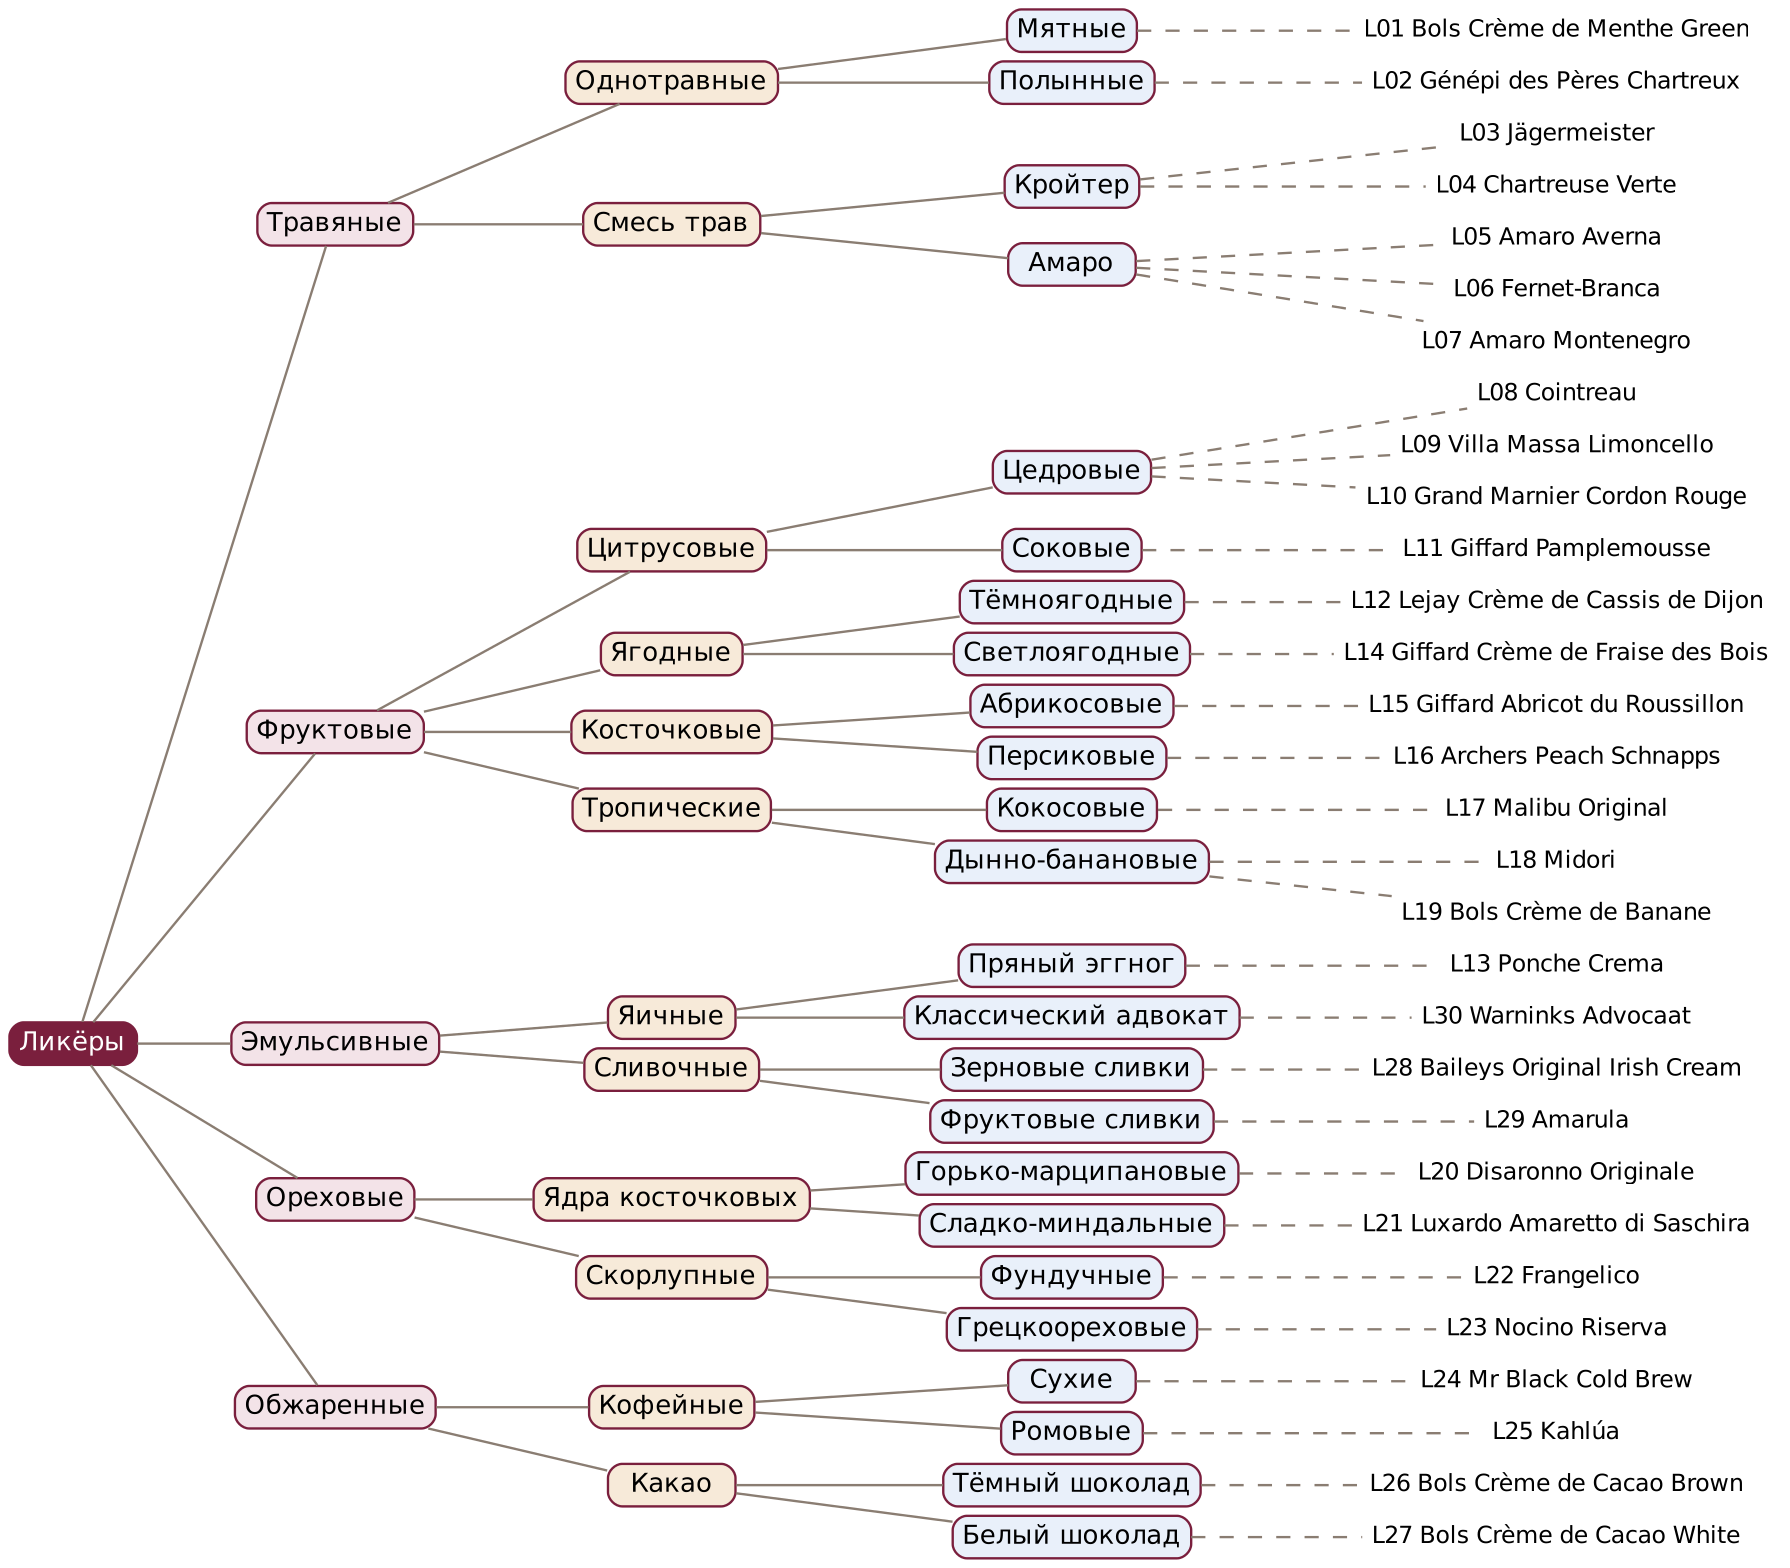
\includegraphics[width=\textwidth]{diags/taxonomy.png}
	\caption{Иерархия предметной области. Сплошные рёбра --- таксономия вкуса, пунктир --- объекты датасета}
	\label{fig:lr1_tree}
\end{figure}

\textbf{Почему основа деления --- вкус.} Рассматривались и другие варианты основания дерева.
\begin{itemize}[leftmargin=1.6\parindent, label*=---]
	\item \textit{По крепости или сладости} с рубежами вроде <<до 20\,\%>> или <<20--30\,\%>>. Вариант отвергнут. Крепость и сладость --- числовые признаки объекта, а не смысловое деление. По методическим указаниям числовые признаки анализируются в мерах близости и фильтрах поиска, а не в дереве. Кроме того, граница искусственна. Ликёры с 19 и 21\,\% оказались бы в разных ветвях.
	\item \textit{По стране.} Отвергнуто, потому что страна --- плоский номинальный признак без внутренней структуры. Одна страна объединяет совершенно разные напитки. Италия --- это и горький Fernet-Branca, и сладкий Limoncello.
	\item \textit{По базовому спирту} --- зерновому, виноградному или ромовому. Отвергнуто, так как для большинства ликёров база не определяет вкус и не известна покупателю.
\end{itemize}
Вкусовая основа --- главный критерий выбора ликёра. Ветви дерева совпадают с тем, как покупатель формулирует желание вроде <<хочу что-то травяное>>. Поэтому вкусовая иерархия выбрана основой классификации, а мера по этому дереву получила в ЛР2 наибольший вес.

\textbf{Почему все листья на одной глубине.} Все вкусовые листья находятся на уровне L3, даже если у группы L2 мало представителей. Одинаковая глубина делает расстояние по дереву сравнимым для любых пар. Мера У--Палмера применяется без поправок на неравномерную глубину, что описано в разделе~\ref{sec:lr2_taxonomy}. Деление на L2 выбрано по значимому признаку производства и вкуса. В травяной ветви это одна трава или сбор трав, во фруктовой --- тип плода, в эмульсивной --- яичная или сливочная основа.

\section{Признаки объектов}
\label{sec:lr1_features}

Набор признаков и их типы приведены в таблице~\ref{tab:lr1_features}. По требованиям ЛР1 нужен хотя бы один бинарный, один количественный, один категориальный и один не приводимый к числовым признак. Датасет содержит их все.

\begin{table}[H]
	\centering
	\caption{Признаки объекта и их роль в системе}
	\label{tab:lr1_features}
	\footnotesize
	\begin{tabular}{|L{2.9cm}|L{3.4cm}|L{3.1cm}|L{4.3cm}|}
		\hline
		Признак & Тип & Значения & Использование \\ \hline
		\code{abv\_pct} & количественный & 15--55 \% & мера (евклидова), фильтр-диапазон \\ \hline
		\code{sugar\_gpl} & количественный & 80--400 г/л & мера (евклидова), фильтр-диапазон \\ \hline
		\code{volume\_l} & количественный & 0,5--1,0 л & мера (евклидова), фильтр-диапазон \\ \hline
		\code{bitter} & бинарный & да / нет & мера SMC, фильтр <<горечь>> \\ \hline
		\code{wood\_contact} & бинарный & да / нет & мера SMC, фильтр <<дерево>> \\ \hline
		\code{sugar\_class} & категориальный порядковый, лингвистическая переменная & малосладкий, умеренный, сладкий, cr\`eme & порядковая мера, фильтр по термам \\ \hline
		\code{taste} (L1/L2/L3) & иерархический, метка класса & 24 листа дерева & мера У--Палмера, фильтр по узлам дерева \\ \hline
		\code{country} & номинальный & 12 стран & $\delta$-функция, фильтр \\ \hline
		\code{producer} & номинальный & 24 производителя & $\delta$-функция, фильтр, текстовый поиск \\ \hline
		\code{name}, \code{notes} & не приводимые к числовым, текст & свободный текст & текстовый поиск и отображение, в меру не входят \\ \hline
		\code{id}, \code{source\_quality} & служебные & --- & идентификация, происхождение данных \\ \hline
	\end{tabular}
\end{table}

Обоснование отдельных признаков приведено ниже.
\begin{itemize}[leftmargin=1.6\parindent, label*=---]
	\item \textbf{Крепость и сахар} --- основные количественные характеристики вкуса ликёра. Значения сахара меняются от 80 г/л у сухого Fernet-Branca до 400 г/л у кремовых ликёров. Объём бутылки --- слабый, но объективный признак. Литровые и полулитровые бутылки характерны для определённых стилей вроде сливочных и альпийских. В мере ЛР2 объём остаётся одной из трёх равноправных числовых осей.
	\item \textbf{Бинарные признаки} определены строго, чтобы их значение не зависело от вкуса эксперта. Признак \code{bitter} означает выраженную структурную горечь. Горечь ментола у мятного ликёра не считается. Признак \code{wood\_contact} означает выдержку ликёра в бочке или выдержанный базовый спирт, как коньяк в Grand Marnier или виски в Baileys.
	\item \textbf{Класс сладости} --- лингвистическая переменная над \code{sugar\_gpl} с четырьмя термами. Малосладкий --- менее 200 г/л, умеренный --- 200--250, сладкий --- 250--350, cr\`eme --- от 350 г/л. Порог 250 г/л взят из регламента ЕС. Начиная с него ликёр может называться <<cr\`eme de\ldots>>~\cite{eu-spirits}. Это категориальный признак, приводимый к числовой шкале, как и предусмотрено заданием. Он нужен, чтобы пользователь мог задавать сладость словами в фильтре ЛР4, а мера мягче различала соседние термы.
	\item \textbf{Текстовые признаки} --- название и описание --- к числам не приводятся. В меру близости они не входят. На 30 объектах нельзя надёжно оценить семантическую близость описаний, а word2vec-модели требуют большого корпуса. Название используется в текстовом поиске ЛР4.
\end{itemize}

\section{Датасет}

Датасет хранится в файле \code{1-dataset/dataset.json} и приведён в таблице~\ref{tab:lr1_dataset}. Копия для просмотра сохранена в \code{liqueurs\_dataset\_30.xlsx}. Формат JSON выбран потому, что признак \code{taste} --- вложенная структура с уровнями L1, L2, L3 и кодом пути. JSON сохраняет её и типы значений без дополнительного разбора. Описание полей и правила построения лингвистической переменной хранятся в том же файле, поэтому датасет самодокументирован.

\vspace{4mm}
{\renewcommand{\arraystretch}{0.72}\setlength{\tabcolsep}{2pt}
\begin{longtable}{|S{0.7cm}|S{4.0cm}|S{2.3cm}|S{2.8cm}|S{0.7cm}|S{0.7cm}|S{0.7cm}|S{0.35cm}|S{0.35cm}|S{1.9cm}|}
	\caption{Датасет из 30 ликёров. Г --- горечь, Д --- контакт с деревом}\label{tab:lr1_dataset}\\ \hline
	ID & Название & Страна & Лист L3 & \% & г/л & л & Г & Д & Класс \\ \hline
	\endfirsthead
	\multicolumn{10}{l}{Продолжение таблицы~\ref{tab:lr1_dataset}} \\ \hline
	ID & Название & Страна & Лист L3 & \% & г/л & л & Г & Д & Класс \\ \hline
	\endhead
L01 & Bols Cr\`eme de Menthe Green & Нидерланды & Мятные & 24 & 400 & 0,7 & -- & -- & cr\`eme \\ \hline
L02 & G\'en\'epi des P\`eres Chartreux & Франция & Полынные & 40 & 200 & 0,5 & + & -- & умеренный \\ \hline
L03 & J\"agermeister & Германия & Кройтер & 35 & 136 & 0,7 & + & -- & малосладкий \\ \hline
L04 & Chartreuse Verte & Франция & Кройтер & 55 & 250 & 0,7 & + & -- & сладкий \\ \hline
L05 & Amaro Averna & Италия & Амаро & 29 & 230 & 0,7 & + & + & умеренный \\ \hline
L06 & Fernet-Branca & Италия & Амаро & 39 & 80 & 0,7 & + & -- & малосладкий \\ \hline
L07 & Amaro Montenegro & Италия & Амаро & 23 & 220 & 0,7 & + & -- & умеренный \\ \hline
L08 & Cointreau & Франция & Цедровые & 40 & 200 & 0,7 & -- & -- & умеренный \\ \hline
L09 & Villa Massa Limoncello & Италия & Цедровые & 30 & 320 & 0,7 & -- & -- & сладкий \\ \hline
L10 & Grand Marnier Cordon Rouge & Франция & Цедровые & 40 & 214 & 0,7 & -- & + & умеренный \\ \hline
L11 & Giffard Pamplemousse & Франция & Соковые & 16 & 260 & 0,7 & -- & -- & сладкий \\ \hline
L12 & Lejay Cr\`eme de Cassis de Dijon & Франция & Тёмноягодные & 20 & 400 & 0,7 & -- & -- & cr\`eme \\ \hline
L13 & Ponche Crema & Венесуэла & Пряный эггног & 15 & 240 & 0,75 & -- & -- & умеренный \\ \hline
L14 & Giffard Cr\`eme de Fraise des Bois & Франция & Светлоягодные & 16 & 380 & 0,7 & -- & -- & cr\`eme \\ \hline
L15 & Giffard Abricot du Roussillon & Франция & Абрикосовые & 25 & 280 & 0,7 & -- & -- & сладкий \\ \hline
L16 & Archers Peach Schnapps & Великобритания & Персиковые & 18 & 280 & 0,7 & -- & -- & сладкий \\ \hline
L17 & Malibu Original & Барбадос & Кокосовые & 21 & 180 & 0,7 & -- & -- & малосладкий \\ \hline
L18 & Midori & Япония & Дынно-банановые & 20 & 300 & 0,7 & -- & -- & сладкий \\ \hline
L19 & Bols Cr\`eme de Banane & Нидерланды & Дынно-банановые & 17 & 400 & 0,7 & -- & -- & cr\`eme \\ \hline
L20 & Disaronno Originale & Италия & Горько-марципановые & 28 & 300 & 0,7 & -- & -- & сладкий \\ \hline
L21 & Luxardo Amaretto di Saschira & Италия & Сладко-миндальные & 28 & 280 & 0,7 & -- & -- & сладкий \\ \hline
L22 & Frangelico & Италия & Фундучные & 20 & 240 & 0,7 & -- & -- & умеренный \\ \hline
L23 & Nocino Riserva & Италия & Грецкоореховые & 30 & 220 & 0,5 & + & + & умеренный \\ \hline
L24 & Mr Black Cold Brew & Австралия & Сухие & 25 & 160 & 0,7 & + & -- & малосладкий \\ \hline
L25 & Kahl\'ua & Мексика & Ромовые & 16 & 393 & 0,7 & -- & -- & cr\`eme \\ \hline
L26 & Bols Cr\`eme de Cacao Brown & Нидерланды & Тёмный шоколад & 24 & 395 & 0,7 & -- & -- & cr\`eme \\ \hline
L27 & Bols Cr\`eme de Cacao White & Нидерланды & Белый шоколад & 24 & 395 & 0,7 & -- & -- & cr\`eme \\ \hline
L28 & Baileys Original Irish Cream & Ирландия & Зерновые сливки & 17 & 224 & 1 & -- & + & умеренный \\ \hline
L29 & Amarula & ЮАР & Фруктовые сливки & 17 & 200 & 0,75 & -- & + & умеренный \\ \hline
L30 & Warninks Advocaat & Нидерланды & Классический адвокат & 17,2 & 260 & 0,7 & -- & -- & сладкий \\ \hline
\end{longtable}
}

\section*{Выводы}
\addcontentsline{toc}{section}{Выводы}

Сформирован датасет из 30 ликёров с признаками пяти типов. Это количественные, бинарные, порядковые, номинальные и текстовые признаки. Построена иерархия предметной области по вкусовой основе. В ней 42 узла классификации и 30 объектов при высоте 5 уровней. Все вкусовые листья лежат на одной глубине. Числовые признаки оставлены атрибутами объектов, а не узлами дерева. Это определило схему ЛР2. Дерево сравнивается древесной мерой, а остальные признаки --- своими частными мерами.
